\documentclass[]{article}
\usepackage{geometry}   % my added package "geometry"
\geometry{letterpaper,tmargin=1in,bmargin=1in,lmargin=2.2cm,rmargin=2.2cm}
\usepackage[colorlinks,bookmarksopen,bookmarksnumbered,
citecolor=green,urlcolor=red]{hyperref}
\hypersetup{pdfauthor={Name}}
%%%%%%%%%%%%%%%%%%%%%%%%%%%%%%%%%%%%%%%%%%%%%%%%%%%%%%%%%%%%%%%%%%%%%%%%%
%\usepackage{graphicx}
\usepackage{graphics}
\usepackage{epsfig}
\usepackage{epstopdf}
\usepackage{amsfonts}
\usepackage{amssymb}
\usepackage{booktabs}
\usepackage{color,soul}
\usepackage{subfig}
%%%%%%%%%%%%%%%%%%%%%%%%%%%%%%%%%%%%%%%%%%%%%%%%%%%%%%%%%%%%%%%%%
\usepackage{amsmath}
\usepackage{cleveref}
\usepackage{authblk}
%\usepackage[fleqn]{amsmath}
\usepackage{lineno}
\usepackage{tikz}
\usepackage{standalone}
\usetikzlibrary{calc,patterns,arrows.meta,shapes.arrows,intersections,positioning}
\usetikzlibrary{decorations.pathmorphing,backgrounds,fit,petri}
\usepackage[percent]{overpic}
%%%%%%%%%%%%%%%%%%%%%%%%%%%%%%%%%%%%%%%%%%%%%%%%%%%%%%%%%%%%%%%%%
\usepackage{xcolor}
\usepackage{listings}
\lstset { %
	language=C++,
	backgroundcolor=\color{blue!5}, % set backgroundcolor
	basicstyle=\footnotesize\color{black},% basic font settingbasicstyle=\ttfamily\color{black}
	keywordstyle=\color{red},
	commentstyle=\color{violet},
	stringstyle=\color{blue},
	xleftmargin=2em,
	frame=single,
	framexleftmargin=2em,
	numbers=left,
	numberstyle=\tiny,
	numbersep=8pt,
}
%%%%%%%%%%%%%%%%%%%%%%%%%%%%%%%%%%%%%%%%%%%%%%%%%%%%%%%%%%%%%%%%%
\renewcommand\thesubsection{\thesection\Alph{subsection}}
%%%%%%%%%%%%%%%%%%%%%%%%%%%%%%%%%%%%%%%%%%%%%%%%%%%%%%%%%%%%%%%%%
\renewcommand\lstlistingname{Header}
\renewcommand\lstlistlistingname{Header}
%%%%%%%%%%%%%%%%%%%%%%%%%%%%%%%%%%%%%%%%%%%%%%%%%%%%%%%%%%%%%%%%%%%%
%opening
\begin{document}
\title{HiperLife Tutorial: Cavity flow (Steady Navier-Stokes)}
\author{Arash Imani}
\affil{LaCàN}
\maketitle

\linenumbers

\section{Problem Definition} \label{sec: pd} 
A number of important phenomena in fluid mechanics are described by the Navier-Stokes equations. They are a statement of the dynamical effect of the externally applied forces and the internal forces of a fluid that we shall assume Newtonian. The internal forces are due to the pressure and the viscosity of the fluid.
Then, the time-dependent flow of a viscous incompressible fluid is governed by the following form of the momentum equation and the mass-conservation equation, called the Navier-Stokes equations:\cite{donea2003finite}
\begin{equation}\label{eq1}
	\begin{aligned}
		&-\nabla \cdot \boldsymbol\upsilon = 0\thinspace,\\
		&\rho \Big( \frac{\partial \boldsymbol\upsilon}{\partial t } + (\boldsymbol\upsilon \cdot \nabla) \boldsymbol\upsilon \Big) + \nabla p - \mu \nabla \cdot \Big[(\nabla \boldsymbol\upsilon) + (\nabla \boldsymbol\upsilon^T)  \Big]= \rho \mathbf{b}\thinspace.
	\end{aligned}
\end{equation}
Here, $\rho$ is the fluid density and $\mathbf{b}$ the volume force per unit mass of fluid, and $\mu$ is dynamic viscosity of the fluid ($Pa\cdot s$). Here we are going to solve the exact same cavity flow problem but for Navier-Stokes formulation. Figure \ref{fig_SB} shows a schematic representation of the problem. It models a plane flow of an isothermal fluid in a square lid-driven cavity. The upper side of the cavity moves in its own plane at unit speed, while the other sides are fixed.

\begin{figure}[htbp]
	\centering
	
\documentclass[preprint,12pt,a4]{standalone}
\usepackage{geometry}   % my added package "geometry"
\geometry{letterpaper,tmargin=1in,bmargin=1in,lmargin=2.5cm,rmargin=2.5cm}
\usepackage{tikz}
\usetikzlibrary{calc,patterns,arrows.meta,shapes.arrows,intersections,positioning}
\usetikzlibrary{decorations.pathmorphing,backgrounds,fit,petri}
\usepackage{standalone}
\begin{document}
	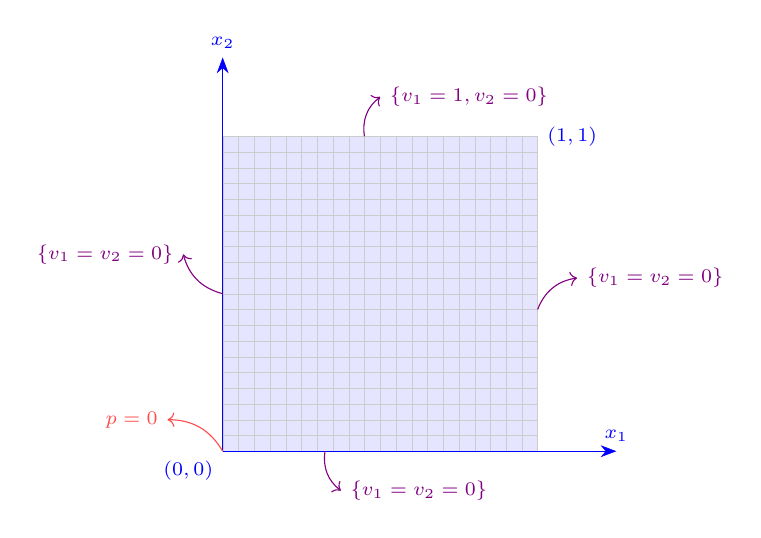
\begin{tikzpicture} [{place/.style={rectangle,draw=blue!50,fill=blue!20,ultra thin,inner sep=0.8mm}},{place2/.style={circle,draw=black!50,ultra thin,inner sep=0.8mm}},{linest/.style={color=gray,ultra thin}}]
	%%coordinates of corners of Beam
	\coordinate (A) at (0,0);
	\coordinate (B) at (4.0,0);
	\coordinate (D) at (4.0,4.0);
	\coordinate (E) at (0.0,4.0);
	
	%% fluid
	\draw [gray!30,fill=blue!10](A) rectangle (D)node [right,color = blue,font=\scriptsize] {$(1,1)$};
	%%mesh
	\draw [line width=0.1pt,gray!40,step=2mm](0,0) grid (D);

	%%axes
	\draw [-{Stealth[length=2mm]},help lines,blue] ($(0,0)$)node [below left,color = blue,font=\scriptsize] {$(0,0)$} -> ($(B)+(1,0)$) node [above,color = blue,font=\scriptsize] {$x_1$};
	\draw [-{Stealth[length=2mm]}, help lines,blue] ($(0,0)$) -> ($(D)+(-4,1)$) node [above,color = blue,font=\scriptsize] {$x_2$};
	

	%%BC
	%% velocity
	\draw [->,violet] (4,1.8) to [bend left] (4.5,2.2)node [right,color = violet,font=\scriptsize] {\{$v_1=v_2=0\}$};
	
	\draw [->,violet] (1.8,4) to [bend left] (2.0,4.5)node [right,color = violet,font=\scriptsize] {\{$v_1=1, v_2=0\}$};
	
	\draw [->,violet] (0,2.0) to [bend left] (-0.5,2.5)node [left,color = violet,font=\scriptsize] {\{$v_1=v_2=0\}$};
	
	\draw [->,violet] (1.3,0) to [bend right] (1.5,-0.5)node [right,color = violet,font=\scriptsize] {\{$v_1=v_2=0\}$};
	%% pressure
	\draw [->,red!70] (0.0,0.0) to [bend right] (-0.7,0.4)node [left,color = red!70,font=\scriptsize] {$p=0$};
	\end{tikzpicture}
\end{document}
	\caption{Geometry, boundary conditions and computational domain used for the analysis.}
	\label{fig_SB}
\end{figure}
\section{Governing Equation} \label{sec: GE} 
Introducing the Reynolds number as
\begin{equation}\label{eq2}
	\begin{aligned}
		Re = \frac{\rho VL}{\mu} = \frac{VL}{\nu}\thinspace.
	\end{aligned}
\end{equation}
where $\nu$ denotes the kinematic viscosity of the fluid ($m^2/s$) and $L$ and $V$ are characteristic of the length and velocity scales of the flow, and dividing both sides of Eq. (\ref{eq1}) by $V^2/L$, allows us to rewrite it in a dimensionless form:
\begin{equation}\label{eq3}
	\begin{aligned}
		&-\nabla \cdot \mathbf{v} = 0\thinspace,\\
		& \frac{\partial \mathbf{v}}{\partial t } + (\mathbf{v} \cdot \nabla) \mathbf{v}  + \nabla P - \frac{1}{Re} \nabla \cdot \Big[(\nabla \mathbf{v}) + (\nabla \mathbf{v}^T)  \Big]=  \mathbf{f}\thinspace.
	\end{aligned}
\end{equation}
where the $x =x/L$ and $\mathbf{v}= \boldsymbol{\upsilon}/V$ and $P = p/\rho V^2$ and $f=\mathbf{b}(L/V^2)$ and $t=t(V/L)$ . The boundary conditions for the flow problem are
given by
\begin{equation}\label{eq4}
	\begin{aligned}
		\mathbf{v} = \mathbf{\bar{v}} \quad \mathrm{on} \ \Gamma_D\thinspace,\\
		\mathbf{t} \equiv \mathbf{\hat{n}} \cdot \boldsymbol{\sigma} = \mathbf{\hat{t}} \quad \mathrm{on} \ \Gamma_N\thinspace.
	\end{aligned}
\end{equation}
where $\mathbf{\hat{n}}$ is the unit normal to the boundary and $\mathbf{\hat{t}}$ is the traction.  The Cauchy stress tensor $\boldsymbol{\sigma}$ can be define as 
\begin{equation}\label{eq5}
	\begin{aligned}
		\boldsymbol{\sigma} = 2\mu \mathbf{D} - P \mathbf{I}
	\end{aligned}
\end{equation}
where $\mathbf{D} = \frac{1}{2} [(\nabla \mathbf{v}) + (\nabla \mathbf{v}^T)]$ and $\mathbf{I}$ is the unit tensor.
\section{Weak Form} \label{sec: WF}
The starting point for the development of the finite element models of Eq. (\ref{eq3}) is their weak forms. Here we consider steady flow ($\frac{d \mathbf{v}}{d t} =0$ ) two-dimensional
case.  The variation formulation of our model problem can be introduced as find $(\mathbf{v},p) \in W$ such that
\begin{equation}\label{eq6}
	\begin{aligned}
		\mathcal{F}(\mathbf{v},P;\mathbf{u},q) = 0 \quad \forall (\mathbf{u},q) \in \hat{W}\thinspace.
	\end{aligned}
\end{equation}
where $W= V \times P$ is a mixed function space, and 
\begin{equation}\label{eq7}
	\begin{aligned}
		\mathcal{F}(\mathbf{v},p;\mathbf{u},q) =\int_{\Omega}  \mathbf{u}(\mathbf{v} \cdot \nabla) \mathbf{v} + \mathbf{u} \nabla P -\frac{1}{Re}\mathbf{u} \nabla \cdot \Big[(\nabla \mathbf{v}) + (\nabla \mathbf{v})^T  \Big] - q \nabla \cdot \mathbf{v} - \mathbf{u} \mathbf{f}\ \mathrm{d}\Omega \thinspace .
	\end{aligned}
\end{equation}
and
\begin{equation}\label{eq8}
	\begin{aligned}
		\hat{W} &= \{\mathbf{u} \in H^1(\Omega) : \mathbf{u} = 0 \text{ on } \Gamma\}, \\
		W &= \{\mathbf{u} \in H^1(\Omega) : \mathbf{u} = 0 \text{ on } (x=0,x=1,y=0), u_2 = 1 \text{ on } y=1 \}\thinspace.
	\end{aligned}
\end{equation}
where $(\mathbf{u},q)$ is a test functions, which will be equated, in the our FE model to the interpolation function used for $(\mathbf{v},P)$. Applying integration by part, and using the definition of stress, we can rewrite the weak form as following
\begin{equation}\label{eq9}
	\begin{aligned}
		\mathcal{F}(\mathbf{v},p;\mathbf{u},q) =&\int_{\Omega^e} \mathbf{u}(\mathbf{v} \cdot \nabla) \mathbf{v}+\mathbf{u}\nabla P - \frac{1}{Re}\mathbf{u} \nabla \cdot \Big[(\nabla \mathbf{v}) + (\nabla \mathbf{v}^T)  \Big]
		- \mathbf{u} \mathbf{f} \mathrm{d}V -\int_{\Omega^e} q \nabla \cdot\mathbf{v} \mathrm{d}V\\
		=&\int_{\Omega^e} \Big\{\mathbf{u}(\mathbf{v} \cdot \nabla) \mathbf{v}\Big\} + \Big\{\nabla \cdot [\mathbf{u}P] - P\nabla  \mathbf{u} \Big\} + \Big\{\frac{1}{Re}\nabla \mathbf{u} \cdot\Big[(\nabla \mathbf{v}) + (\nabla \mathbf{v})^T  \Big] - \nabla \cdot \Big(2\mathbf{u}\mu \mathbf{D} \Big) \Big\} - \mathbf{u} \mathbf{f}\mathrm{d}V\\
		 &-\int_{\Omega^e} q \nabla \cdot\mathbf{v} \mathrm{d}V \\
		=&\int_{\Omega^e} \mathbf{u}(\mathbf{v} \cdot \nabla) \mathbf{v}\mathrm{d}V + \int_{\Gamma^e} \mathbf{u}P \mathbf{I} \cdot \mathbf{n} \mathrm{d}S
		-\int_{\Omega^e}P\nabla  \mathbf{u} \mathrm{d}V
		-\int_{\Gamma^e} (2\mathbf{u}\mu \mathbf{D}) \cdot \mathbf{n} \mathrm{d}S
		+\int_{\Omega^e}\frac{1}{Re} \nabla\mathbf{u}\cdot\Big[(\nabla \mathbf{v}) + (\nabla \mathbf{v})^T  \Big] \mathrm{d}V\\
		&-\int_{\Omega^e}\mathbf{u} \mathbf{f} \mathrm{d}V - \int_{\Omega^e} q \nabla \cdot \mathbf{v} \mathrm{d}V \\ 
		=&-\int_{\Gamma^e} \mathbf{u} \mathbf{\hat{t}}\mathrm{d}S
		+\int_{\Omega^e} \mathbf{u}(\mathbf{v} \cdot \nabla) \mathbf{v} + \frac{1}{Re} \nabla \mathbf{u} \Big[(\nabla \mathbf{v}) + (\nabla \mathbf{v})^T  \Big] - P\nabla \mathbf{u} - \mathbf{u} \mathbf{f}\mathrm{d}V - \int_{\Omega^e} q \nabla \cdot \mathbf{v} \mathrm{d}V \thinspace.
	\end{aligned}
\end{equation}
Since $	\mathcal{F}$ is a nonlinear function of $\mathbf{v}$, the variational statement gives rise to a system of nonlinear algebraic equations.we now need to linearize it, we may use Newton’s method to solve the system of nonlinear algebraic equations. Newton’s method for the system $\mathcal{F}(V_1,\ldots,V_j)$ can be formulated by the first terms of a Taylor series approximation for the value of the variational as
\begin{equation}\label{eq10}
	\begin{aligned}
		\sum_{j=1}^N {\partial \over\partial V_j} \mathcal{F}(V_1^k,\ldots,V_N^k)\delta V_j &= -\mathcal{F}(V_1^k,\ldots,V_N^k),\quad i=1, \ldots ,N,\\ V_j^{k+1} &= V_j^k + \delta V_j,\quad j=1, \ldots ,N,
	\end{aligned}
\end{equation}
where $k$ is an iteration index. An initial guess $\mathbf{v}^0$ must be provided to start the algorithm. We need to compute the $\partial \mathcal{F}/\partial V_j$ and the right-hand side vector $-\mathcal{F}$. Our present problem has $\mathcal{F}$ given by above.
\begin{equation}\label{eq11}
	\begin{aligned}
		{\partial F\over\partial V_j} = \int_\Omega \mathbf{u} \Big(\frac{\partial \mathbf{v}}{\partial V_j}\cdot\nabla\Big) \mathbf{v}  + \mathbf{u}\Big(\mathbf{v} \cdot \nabla\Big) [\frac{\partial \mathbf{v}}{\partial V_j}] + \frac{1}{Re} \nabla \mathbf{u} \Big[\nabla[\frac{\partial \mathbf{v}}{\partial V_j}] + (\nabla[\frac{\partial \mathbf{v}}{\partial V_j}])^T]\Big] - q \nabla \cdot (\frac{\partial \mathbf{v}}{\partial V_j}) \mathrm{d}\Omega\thinspace .
	\end{aligned}
\end{equation}
by adding the pressure term, Hessian is given by
\begin{equation}\label{eq11}
	\begin{aligned}
		\mathcal{J}(\mathbf{v},p;\mathbf{u},q) = \int_\Omega \mathbf{u} \Big(\frac{\partial \mathbf{v}}{\partial V_j}\cdot \nabla\Big) \mathbf{v}  + \mathbf{u}\Big(\mathbf{v} \cdot \nabla\Big) [\frac{\partial \mathbf{v}}{\partial V_j}] + \frac{1}{Re} \nabla \mathbf{u} \Big[\nabla[\frac{\partial \mathbf{v}}{\partial V_j}] + (\nabla[\frac{\partial \mathbf{v}}{\partial V_j}])^T]\Big] - q \nabla \cdot (\frac{\partial \mathbf{v}}{\partial V_j}) - \frac{\partial P}{\partial P_j}\nabla \mathbf{u}\mathrm{d}\Omega\thinspace .
	\end{aligned}
\end{equation}

\section{Finite Element Model} \label{sec: FEM}
Since we are developing the Ritz-Galerkin finite element models, the choice
of the weight functions is restricted to the spaces of approximation functions
used for the pressure and velocity fields. Suppose that the dependent variables
$(v_i, P )$ are approximated by expansions of the form
\begin{equation}\label{eq12}
	\begin{aligned}
		&v_i(\mathrm{x}, t)= \sum_{m=1}^{M} \psi_m(\mathrm{x}) \mathbf{v}_i^m(t) = \boldsymbol{\Psi}^T\mathbf{V}_i \thinspace,\\
		&p(\mathrm{x}, t)= \sum_{n=1}^{N} \phi_n(\mathrm{x}) P^n(t) = \boldsymbol{\Phi}^T\mathbf{P} \thinspace.
	\end{aligned}
\end{equation}
where $\boldsymbol{\Psi}$ and $\boldsymbol{\Phi}$ are vectors of interpolation (or shape) functions, $\mathbf{V}^{k+1} = \{v_1,v_2\}^T$ and
$\mathbf{P}$ are vectors of nodal values of velocity components and pressure, respectively. Substitution of these equation into Eq. (\ref{eq11}) results in the following finite element equation.

\begin{equation}\label{eq14}
	\begin{aligned}
		\mathcal{J} =& \Big[\int_{\Omega^e} \boldsymbol{\Psi} \Big(\boldsymbol{\Psi} \cdot\nabla\Big) \mathbf{v}^k  \mathrm{d}\Omega\Big] \mathbf{V}
		+ \Big[\int_{\Omega^e}  \boldsymbol{\Psi} \Big(\mathbf{v}^k \cdot \nabla\Big) \boldsymbol{\Psi}\mathrm{d}\Omega\Big] \mathbf{V}
		+ \Big[\int_{\Omega^e}  \frac{1}{Re} \nabla \boldsymbol{\Psi} \Big[(\nabla \boldsymbol{\Psi}) +  (\nabla\boldsymbol{\Psi})^T\Big]\mathrm{d}\Omega \Big] \mathbf{V}\\
		&-\Big[\int \boldsymbol{\Phi} \nabla \cdot\boldsymbol{\Psi}  \mathrm{d}V \Big]\mathbf{V}
		-\Big[\int \boldsymbol{\Phi} \nabla \boldsymbol{\Psi}  \mathrm{d}V \Big]\mathbf{P} \thinspace.
	\end{aligned}
\end{equation}
and 
\begin{equation}\label{eq11}
	\begin{aligned}
		\mathcal{F} = \int_{\Omega^e} \boldsymbol{\Psi}\mathbf{v}^k \cdot \nabla \mathbf{v}^k + \frac{1}{Re} \nabla \boldsymbol{\Psi} \Big[(\nabla \mathbf{v}^k) + (\nabla \mathbf{v}^k)^T  \Big] - P^k\nabla \boldsymbol{\Psi}\mathrm{d}V  - \int_{\Omega^e}q \nabla \cdot v^k \mathrm{d}V \thinspace.
	\end{aligned}
\end{equation}
The above equations can be written in a matrix form as

\begin{equation}\label{eq15}
	\begin{aligned}
		-\mathbf{Q}^T \mathbf{v} &= \mathbf{0}\thinspace,\\
		\mathbf{K}\mathbf{v} - \mathbf{Q} \mathbf{P}  &= \mathbf{F}\thinspace.
	\end{aligned}
\end{equation}
By combining continuity and  momentum equations into one, Eq. (\ref{eq8}) has the following explicit matrix form:
\begin{equation}\label{eq16}
	\begin{aligned}
		\begin{bmatrix}
			\mathbf{C}_{11} & \mathbf{C}_{12} & 0 \\
			\mathbf{C}_{21} & \mathbf{C}_{22} &  0\\
			 0& 0  & 0 \\
		\end{bmatrix}
		\begin{Bmatrix}
			\mathbf{v_1} \\
			\mathbf{v_2}\\
			\mathbf{P}\\
		\end{Bmatrix}
		+\begin{bmatrix}
			2\mathbf{K}_{11} + \mathbf{K}_{22} & \mathbf{K}_{12} & -\mathbf{Q}_{1} \\
			\mathbf{K}_{21} & \mathbf{K}_{11} +2\mathbf{K}_{22} & -\mathbf{Q}_{2} \\
			-\mathbf{Q}^T_{1} & -\mathbf{Q}^T_{2}  & \mathbf{0} \\
		\end{bmatrix}
		\begin{Bmatrix}
			\mathbf{v_1} \\
			\mathbf{v_2}\\
			\mathbf{P}\\
		\end{Bmatrix}
			=\begin{Bmatrix}
				\mathbf{F_1} \\
				\mathbf{F_2}\\
				\mathbf{F_3}\\
			\end{Bmatrix}\thinspace.
	\end{aligned}
\end{equation}
The coefficient matrices shown in Eq. (\ref{eq9}) are defined by
\begin{equation}\label{eq13}
	\begin{aligned}
		&\mathbf{K}_{ij} = \int_{\Omega^e} \nu \frac{\partial\boldsymbol{\Psi}}{\partial x_i} \frac{\partial\boldsymbol{\Psi}^T}{\partial x_j}\mathrm{d}V\thinspace, \quad \mathbf{Q}_i = \int_{\Omega^e}\frac{\partial\boldsymbol{\Psi}}{\partial x_i} \boldsymbol{\Phi}^T \mathrm{d}V\thinspace, \thinspace,\\
		&\mathbf{C}_{11} = \int_{\Omega^e} \boldsymbol{\Psi} \boldsymbol{\Psi}^T \frac{\partial v_1}{\partial x} + \boldsymbol{\Psi} v_1 \frac{\partial \boldsymbol{\Psi}^T}{\partial x} + \boldsymbol{\Psi} v_2 \frac{\partial \boldsymbol{\Psi}^T}{\partial y}\mathrm{d}V\thinspace, \quad
		\mathbf{C}_{12} = \int_{\Omega^e}\boldsymbol{\Psi} \boldsymbol{\Psi}^T \frac{\partial v_1}{\partial y} \mathrm{d}V\thinspace,\\
		&\mathbf{C}_{21} = \int_{\Omega^e} \boldsymbol{\Psi} \boldsymbol{\Psi}^T \frac{\partial v_2}{\partial x}\mathrm{d}V\thinspace,\quad
		\mathbf{C}_{22} = \int_{\Omega^e} \boldsymbol{\Psi} \boldsymbol{\Psi}^T \frac{\partial v_2}{\partial y} + \boldsymbol{\Psi} v_1 \frac{\partial \boldsymbol{\Psi}^T}{\partial x} + \boldsymbol{\Psi} v_2 \frac{\partial \boldsymbol{\Psi}^T}{\partial y}\mathrm{d}V\thinspace.		
	\end{aligned}
\end{equation}
and
\begin{equation}\label{eq15}
	\begin{aligned}
		\mathbf{F}_1 &=\int_{\Omega^e} \boldsymbol{\Psi} v_1 \frac{\partial v_1}{\partial x}
		+ \boldsymbol{\Psi}v_2 \frac{\partial v_1}{\partial y}
		+ \nu  \Big(2\frac{\partial \boldsymbol{\Psi}}{\partial x}\frac{\partial v_1}{\partial x} + \frac{\partial \boldsymbol{\Psi}
		}{\partial y}\Big[\frac{\partial v_1}{\partial y} + \frac{\partial v_2}{\partial x}\Big]\Big) -P \frac{\partial \boldsymbol{\Psi}}{\partial x} \mathrm{d}V,\\
		\mathbf{F}_2 &=\int_{\Omega^e} \boldsymbol{\Psi} v_1 \frac{\partial v_2}{\partial x} 
		+ \boldsymbol{\Psi}v_2 \frac{\partial v_2}{\partial y} 
		+ \nu  \Big(2\frac{\partial \boldsymbol{\Psi}}{\partial y}\frac{\partial v_2}{\partial y} + \frac{\partial \boldsymbol{\Psi}
		}{\partial x} \Big[ \frac{\partial v_1}{\partial y} + \frac{\partial v_2}{\partial x}\Big]\Big) 
		-P \frac{\partial \boldsymbol{\Psi}}{\partial y} \mathrm{d}V,\\
		\mathbf{F}_3 &=\int_{\Omega^e} \boldsymbol{\Phi} \Big(\frac{\partial v_1}{\partial x} + \frac{\partial v_2}{\partial y}\Big)\mathrm{d}V .
	\end{aligned}
\end{equation}
\section{Choice of Elements} \label{sec: elem}
There are lots of elements available for using in mixed finint elements model, but here for sake of simplicity we choose $Q2Q1$ elements. The quadratic quadrilateral elements shown in Figure \ref{fig_elem} are known to give reliable solutions for velocity and pressure fields.
\begin{figure}[htbp]
	\centering
	\documentclass[preprint,12pt,a4]{standalone}
\usepackage{geometry}   % my added package "geometry"
\geometry{letterpaper,tmargin=1in,bmargin=1in,lmargin=2.5cm,rmargin=2.5cm}
\usepackage{tikz}
\usetikzlibrary{calc,patterns,arrows.meta,shapes.arrows,intersections,positioning}
\usetikzlibrary{decorations.pathmorphing,backgrounds,fit,petri}
\usepackage{standalone}
%
\begin{document}
	\begin{tikzpicture} [{place/.style={rectangle,draw=blue!50,fill=blue!20,ultra thin,inner sep=0.8mm}},{place2/.style={rectangle,draw=black!50,ultra thin,inner sep=0.8mm}},{linest/.style={color=gray,ultra thin}}]
		%axes
		\draw [{Stealth[length=2mm]}-{Stealth[length=2mm]}, help lines,blue] (5.0,0)node[above,font=\scriptsize]{$\xi$} -- (0.0,0.0) -- (0.0,5.0)node[right,font=\scriptsize] {$\eta$};
		%%corner nodes
		\node at (0.0,0.0) [place,fill=violet!60] (1) {};
		\node at (4.0,0.0) [place,fill=violet!60] (2) {};
		\node at (4.0,4.0) [place,fill=violet!60] (3) {};
		\node at (0.0,4.0) [place,fill=violet!60] (4) {};
		%%element border
		\draw [-,black] (1) -- (2) -- (3) -- (4) --(1);
		%%middle nodes
		\node at (2.0,0.0) [place2,fill=gray!60] {};
		\node at (4.0,2.0) [place2,fill=gray!60] {};
		\node at (2.0,4.0) [place2,fill=gray!60] {};
		\node at (0.0,2.0) [place2,fill=gray!60] {};
		\node at (2.0,2.0) [place2,fill=gray!60] {};
		\node at (5.5,3.0) [place2,fill=gray!60] {};
		\node at (5.6,3.0) [right,font=\scriptsize]{$\mathrm{nodes \ with} \ \{v_1, v_2$\}};
		\node at (5.5,2.5) [place,fill=violet!60] (4) {};
		\node at (5.6,2.5) [right,font=\scriptsize]{$\mathrm{nodes \ with} \ \{v_1, v_2, P$\}};
		
	\end{tikzpicture}
\end{document}
	\caption{Quadratic quadrilateral element used for the mixed finite element model.}
	\label{fig_elem}
\end{figure}
\section{Implementation} \label{sec: imp}
In this section, we present the implementation of our solution in the Hiperlife. The program is divided into three separate files, main part which we create our problem by the Hiperlife headers, auxiliary header where we introduce parameters and declare our functions, and at last auxiliary file, where we define some functions which provide required matrices like the Hessian and Jacobian.
\subsubsection{CavityFlowNavier.cpp} \label{sec: m.cpp}
\nolinenumbers
\begin{lstlisting}
/*
* Incompressible Navier stokes flow: Cavity flow problem
*/
// cpp headers
#include <iostream>
#include <fstream>
#include <cmath>

// hiperlife headers
#include "hl_Core.h"
#include "hl_Parser.h"
#include "hl_Tensor.h"
#include "hl_TypeDefs.h"  
#include "hl_DOFsHandler.h"
#include "hl_HiPerProblem.h"
#include "hl_FillStructure.h"
#include "hl_ParamStructure.h"
#include "hl_DistributedMesh.h" 
#include "hl_StructMeshGenerator.h" 
#include "hl_GlobalBasisFunctions.h"
#include "hl_LinearSolver_Direct_MUMPS.h"
#include "hl_NonlinearSolver_NewtonRaphson.h"
#include "hl_LinearSolver_Iterative_AztecOO.h"
#include <hl_ConsistencyCheck.h>

// Header to auxiliary functions
#include "AuxCavityFlowNavier.h"

// -------------------------------------------------------------------//
/// -----------------    MAIN FUNCTION     --------------------------///
// -------------------------------------------------------------------//

int main(int argc, char** argv)
{
	using namespace std;
	using namespace hiperlife;
	using namespace hiperlife::Tensor;
	
	// ---------------------------------------------------------------//
	/// *****                 INITIALIZATION                    *****///
	// ---------------------------------------------------------------//
	
	// Initialize MPI
	hiperlife::Init(argc, argv);
	
	// ---------------------------------------------------------------//
	/// *****                   DATA INPUT                      *****///
	// ---------------------------------------------------------------//
	
	// Put parameters in the user structure
	SmartPtr<ParamStructure> paramStr = CreateParamStructure<CavityNParams>();
	
	// Data
	double Re = 100.0;
	paramStr->setRealParameter(CavityNParams::nu, 1.0/Re);
	paramStr->setRealParameter(CavityNParams::f1, 0.0);
	paramStr->setRealParameter(CavityNParams::f2, 0.0);
	
	double nu = paramStr->getRealParameter(CavityNParams::nu);
	double f1 = paramStr->getRealParameter(CavityNParams::f1);
	double f2 = paramStr->getRealParameter(CavityNParams::f2);
	
	
	// analysis parameter
	ElemType elemType = ElemType::Square;// Triang or Square
	int n = 10;// number of elements in x and y direction
	// ---------------------------------------------------------------//
	/// *****                   MESH CREATION                   *****///
	// ---------------------------------------------------------------//
	// Create a structural mesh       
	SmartPtr<StructMeshGenerator> StrMesh = Create<StructMeshGenerator>();
	
	StrMesh->setNDim(3);
	StrMesh->setBasisFuncType(BasisFuncType::Lagrangian);
	StrMesh->setBasisFuncOrder(1);
	StrMesh->setElemType(elemType);
	StrMesh->genSquare(n,1.0);
	
	//-------------------Distributed Mesh------------------------------//
	// For Pressure
	SmartPtr<DistributedMesh> disMeshPress = Create<DistributedMesh>();
	
	disMeshPress->setMesh(StrMesh);
	disMeshPress->setBalanceMesh(true);
	disMeshPress->setElementLocatorEngine(ElementLocatorEngine::BoundingVolumeHierarchy);
	disMeshPress->Update();
	
	// For Velocity
	SmartPtr<DistributedMesh> disMeshVeloc = Create<DistributedMesh>();
	
	disMeshVeloc->setMeshRelation(MeshRelation::pRefin, disMeshPress);
	disMeshVeloc->setPRefinement(1);
	disMeshVeloc->setBalanceMesh(true);
	disMeshVeloc->setElementLocatorEngine(ElementLocatorEngine::BoundingVolumeHierarchy);
	disMeshVeloc->Update();
	
	cout << "--check meshv/p files to see the mesh for velocity and pressure--" << endl;
	disMeshVeloc->printFileLegacyVtk("meshv");
	disMeshPress->printFileLegacyVtk("meshp");
	
	// ---------------------------------------------------------------//
	/// *****               DOFsHANDLER CREATION                *****///
	// ---------------------------------------------------------------//
	
	// DOFHandler
	// For Velocity
	SmartPtr<DOFsHandler> dhandV = Create<DOFsHandler>(disMeshVeloc);
	dhandV ->setNameTag("dhandV");
	dhandV ->setNumDOFs(2);
	dhandV->setDOFs({"vx","vy"});
	dhandV->Update();
	
	// For Pressure
	SmartPtr<DOFsHandler> dhandP = Create<DOFsHandler>(disMeshPress);
	dhandP->setNameTag("dhandP");
	dhandP ->setNumDOFs(1);
	dhandP->setDOFs({"p"});
	dhandP->Update(); 
	cout << "--DOFsHandler for Velocity and Pressure successfully created--" << endl;
	
	
	// ------------------ Boundary conditions------------------------ //
	//---------------------------------------------------------------//
	// Set boundary conditions for the velocity
	//velocities are zero everywhere except at Ymax vx=1
	for (int i = 0; i < disMeshVeloc->loc_nPts(); i++)
	{
		if (disMeshVeloc->isNodeInMAxis(MAxis::Xmin, i, IndexType::Local))
		{
			dhandV->nodeDOFs->setValue("vx",i,IndexType::Local,0.0);
			dhandV->nodeDOFs->setValue("vy",i,IndexType::Local,0.0);
			dhandV->setConstraint("vx",i,IndexType::Local,0.0);
			dhandV->setConstraint("vy",i,IndexType::Local,0.0);
		}
		if (disMeshVeloc->isNodeInMAxis(MAxis::Xmax, i, IndexType::Local))
		{
			dhandV->nodeDOFs->setValue("vx",i,IndexType::Local,0.0);
			dhandV->nodeDOFs->setValue("vy",i,IndexType::Local,0.0);
			dhandV->setConstraint("vx",i,IndexType::Local,0.0);
			dhandV->setConstraint("vy",i,IndexType::Local,0.0);
		}
		if (disMeshVeloc->isNodeInMAxis(MAxis::Ymin, i, IndexType::Local))
		{
			dhandV->nodeDOFs->setValue("vx",i,IndexType::Local,0.0);
			dhandV->nodeDOFs->setValue("vy",i,IndexType::Local,0.0);
			dhandV->setConstraint("vx",i,IndexType::Local,0.0);
			dhandV->setConstraint("vy",i,IndexType::Local,0.0);
		}
		if (disMeshVeloc->isNodeInMAxis(MAxis::Ymax, i, IndexType::Local))
		{
			dhandV->nodeDOFs->setValue("vx",i,IndexType::Local,1.0);
			dhandV->nodeDOFs->setValue("vy",i,IndexType::Local,0.0);
			dhandV->setConstraint("vx",i,IndexType::Local,0.0);
			dhandV->setConstraint("vy",i,IndexType::Local,0.0);
		}
	}
	
	// Set boundary conditions for the pressure
	// Set initial value for the pressure at (0,0) p=0 
	//if (disMeshPress->myRank() == 0)
	dhandP->setBoundaryCondition(0,0,IndexType::Local,0.0);
	
	// Save into nodeDOFS0
	dhandP->nodeDOFs0->setValue(dhandP->nodeDOFs);
	dhandV->nodeDOFs0->setValue(dhandV->nodeDOFs);
	
	// Update
	dhandV->UpdateGhosts();
	dhandP->UpdateGhosts();
	
	// initial condition
	cout << "--check pressure/velocityBC0 file to see the applied BCs--" << endl;
	dhandP->printFileLegacyVtk("pressureBC0");
	dhandV->printFileLegacyVtk("velocityBC0");
	
	// ---------------------------------------------------------------//
	/// *****               HIPERPROBLEM CREATION               *****///
	// ---------------------------------------------------------------//
	
	SmartPtr<HiPerProblem> hiperProbl = Create<HiPerProblem>();
	hiperProbl->setParameterStructure(paramStr);
	hiperProbl->setDOFsHandlers({dhandV, dhandP});
	hiperProbl->setIntegration("IntegCavity", {"dhandV", "dhandP"});
	
	if (elemType==ElemType::Square)
	hiperProbl->setCubatureGauss("IntegCavity", 9);
	else if (elemType==ElemType::Triang)
	hiperProbl->setCubatureGauss("IntegCavity", 3);
	
	hiperProbl->setElementFillings("IntegCavity", LS);
	if (true)
	{
		hiperProbl->setConsistencyDOFs("dhandV", {"vx","vy"});
		hiperProbl->setElementFillings("IntegCavity", ConsistencyCheck<LS>);
		hiperProbl->setConsistencyCheckType(ConsistencyCheckType::Hessian);
	}
	hiperProbl->Update();
	// ---------------------------------------------------------------//
	// ---------------------------------------------------------------//
	/// *****                  SOLVER CREATION                  *****///
	// ---------------------------------------------------------------//
	// Create linear solver direct
	SmartPtr<MUMPSDirectLinearSolver> linSolver = Create<MUMPSDirectLinearSolver>();
	linSolver->setHiPerProblem(hiperProbl);
	linSolver->setVerbosity(MUMPSDirectLinearSolver::Verbosity::Low);
	linSolver->setDefaultParameters();
	linSolver->Update();
	
	// Create non-linear solver
	SmartPtr<NewtonRaphsonNonlinearSolver>nonlSlvr=Create<NewtonRaphsonNonlinearSolver>();
	nonlSlvr->setLinearSolver(linSolver);
	nonlSlvr->setMaxNumIterations(25);
	nonlSlvr->setResTolerance(1.E-8);
	nonlSlvr->setSolTolerance(1.E-8);
	nonlSlvr->setLineSearch(true);
	nonlSlvr->setPrintIntermInfo(true);
	nonlSlvr->setConvRelTolerance(true);
	nonlSlvr->Update();
	
	// ---------------------------------------------------------------//
	/// *****                      SOLVE                        *****///
	// ---------------------------------------------------------------//
	
	// Initial guess
	dhandV->nodeDOFs->setValue(dhandV->nodeDOFs0);
	dhandP->nodeDOFs->setValue(dhandP->nodeDOFs0);
	hiperProbl->UpdateGhosts();
	
	// Solve
	bool converged = nonlSlvr->solve();
	
	// Check convergence
	if (converged)
	{
		// Save solution
		dhandV->nodeDOFs0->setValue(dhandV->nodeDOFs);
		dhandP->nodeDOFs0->setValue(dhandP->nodeDOFs);
		
		// Write results and update solution
		dhandV->printFileLegacyVtk("CavityNavier_v", true);
		dhandP->printFileLegacyVtk("CavityNavier_p", true);
	} else
	{
		throw runtime_error("Error: NonLinear solver did not converge.");
	}
	
	// mpi finilizing
	hiperlife::Finalize();
	return 0;
}
\end{lstlisting}
\subsubsection{AuxCavityFlowNavier.h} \label{sec: a.h}
\begin{lstlisting}
#ifndef AUXCavityN_H
#define AUXCavityN_H

// C headers
#include <iostream>

// hiperlife headers
#include "hl_Core.h"
#include "hl_Parser.h"
#include "hl_TypeDefs.h"  
#include "hl_DOFsHandler.h"
#include "hl_HiPerProblem.h"
#include "hl_FillStructure.h"
#include "hl_ParamStructure.h"
#include "hl_DistributedMesh.h" 
#include "hl_StructMeshGenerator.h" 
#include "hl_GlobalBasisFunctions.h"
#include "hl_NonlinearSolver_NewtonRaphson.h"
#include "hl_LinearSolver_Iterative_AztecOO.h"

struct CavityNParams
{
	enum RealParameters
	{
		nu,
		f1,
		f2,
	};
	HL_PARAMETER_LIST DefaultValues
	{
		{"nu,", 0.01},
		{"f1,", 0.0},
		{"f2,", 0.0},
	};
};

void LS(hiperlife::FillStructure& fillStr);

#endif

\end{lstlisting}
\subsubsection{AuxCavityFlowNavier.cpp} \label{sec: a.cpp}
\begin{lstlisting}
// Header to cpp
#include <fstream>
#include <iostream>
#include <string>

// Header to auxiliary functions
#include "AuxCavityFlowNavier.h"

// Hiperlife headers
#include "hl_Core.h"
#include "hl_ParamStructure.h"
#include "hl_Parser.h"
#include "hl_TypeDefs.h"
#include "hl_GlobalBasisFunctions.h"
#include "hl_StructMeshGenerator.h"
#include "hl_DistributedMesh.h"
#include "hl_FillStructure.h"
#include "hl_DOFsHandler.h"
#include "hl_HiPerProblem.h"
#include "hl_LinearSolver_Iterative_AztecOO.h"
#include "hl_NonlinearSolver_NewtonRaphson.h"

using namespace std;
using namespace hiperlife;
using namespace hiperlife::Tensor;


// Cavity flow

void LS(hiperlife::FillStructure& fillStr)
{
	using namespace std;
	using namespace hiperlife;
	using hiperlife::Tensor::tensor;
	
	double nu = fillStr.getRealParameter(CavityNParams::nu);
	double f1 = fillStr.getRealParameter(CavityNParams::f1);
	double f2 = fillStr.getRealParameter(CavityNParams::f2);
	ttl::tensor<double,1>  F{f1,f2};
	
	
	//----------------------------------------------------------------//
	// ------------------------- INPUT DATA --------------------------//
	//----------------------------------------------------------------//
	
	//--------------------------Velocity-related----------------------//
	// Dimensions
	SubFillStructure& subFill = fillStr["dhandV"];
	int pDim = subFill.pDim;
	int eNN  = subFill.eNN;
	int numDOFs = subFill.numDOFs;
	
	// Shape functions and derivatives at Gauss points
	double jac{};
	ttl::wrapper<double,2> nborCoords(subFill.nborCoords.data(),eNN,pDim);
	ttl::wrapper<double,2> nborDOFs(subFill.nborDOFs.data(),eNN,numDOFs);
	ttl::tensor<double,1,false>  bf(subFill.nborBFs(),eNN);
	ttl::tensor<double,2> Dbf_g(eNN,pDim);
	GlobalBasisFunctions::gradients(Dbf_g, jac, subFill);
	
	//--------------------------Pressure-related----------------------//
	// Dimensions
	SubFillStructure& subFill_p = fillStr["dhandP"];
	int nDim_p = subFill_p.nDim;
	int eNN_p  = subFill_p.eNN;
	int numDOFs_p = subFill_p.numDOFs;
	
	// Shape functions and derivatives at Gauss points
	ttl::wrapper<double,2> nborCoords_p(subFill_p.nborCoords.data(),eNN_p,nDim_p);
	ttl::wrapper<double,1> nborDOFs_p(subFill_p.nborDOFs.data(),eNN_p);
	ttl::tensor<double,1,false>  bf_p(subFill_p.nborBFs(),eNN_p);
	
	//-------------------------------------------------------------------------------//
	// ------------------------------- OUTPUT DATA ----------------------------------//
	//-------------------------------------------------------------------------------//
	ttl::wrapper<double,2> Bk0(fillStr.Bk(0).data(),eNN,numDOFs);
	ttl::wrapper<double,1> Bk1(fillStr.Bk(1).data(),eNN_p);
	
	ttl::wrapper<double,4> Ak00(fillStr.Ak(0,0).data(),eNN,numDOFs,eNN,numDOFs);
	ttl::wrapper<double,3> Ak01(fillStr.Ak(0,1).data(),eNN,numDOFs,eNN_p);
	ttl::wrapper<double,3> Ak10(fillStr.Ak(1,0).data(),eNN_p,eNN,numDOFs);
	ttl::wrapper<double,2> Ak11(fillStr.Ak(1,1).data(),eNN_p,eNN_p);
	
	//-------------------------------- EQUATIONS ------------------------------------//
	//-------------------------------------------------------------------------------//
	tensor<double,1> v  = bf * nborDOFs;
	double  pre = bf_p * nborDOFs_p;
	
	tensor<double,2> Dv = product(nborDOFs,Dbf_g,{{0,0}});
	double divv = trace(Dv);
	
	//tensor form
	// create a 4th order tensor out of Dbf_g
	tensor<double,4> Dbf4 = outer(Dbf_g,Identity(pDim));
	Ak00 += jac * nu * product(Dbf4,Dbf4 + Dbf4.transpose({0,2,1,3}),{{1,1},{2,2}});
	Ak00 += jac * outer(outer(bf,Dv),bf).transpose({0,1,3,2});
	Ak00 += jac * outer(outer(bf,Identity(pDim)),Dbf_g*v).transpose({0,1,3,2});
	
	Ak01 += -jac * outer(Dbf_g,bf_p);
	Ak10 += -jac * outer(bf_p,Dbf_g);
	
	Bk0 += jac * outer(bf,Dv*v);
	Bk0 += -jac * pre * Dbf_g ;
	Bk0 += jac * nu * Dbf_g * (Dv + Dv.T());
	Bk1 += -jac * divv * bf_p;
	
	//indices form
	//for (int i=0;i < eNN;i++)
	//{
		//for (int j=0;j < eNN;j++)
		//{
			//Ak00(i,0,j,0)+=jac*nu*(2.0*Dbf_g(i,0)*Dbf_g(j,0)
			//+Dbf_g(i,1)*Dbf_g(j,1));
			//Ak00(i,0,j,0)+=jac*(bf(i)*Dv(0,0)*bf(j)
			+bf(i)*v(0)*Dbf_g(j,0)+bf(i)*v(1)*Dbf_g(j,1));
			
			//Ak00(i,0,j,1)+=jac*nu*(Dbf_g(i,1)*Dbf_g(j,0));
			//Ak00(i,0,j,1)+=jac*(bf(i)*bf(j)*Dv(0,1));
			
			//Ak00(i,1,j,0)+=jac*nu*(Dbf_g(i,0)*Dbf_g(j,1));
			//Ak00(i,1,j,0)+=jac*(bf(i)*Dv(1,0)*bf(j));
			
			//Ak00(i,1,j,1)+=jac*nu*(2.0*Dbf_g(i,1)*Dbf_g(j,1)
			//+Dbf_g(i,0)*Dbf_g(j,0));
			//Ak00(i,1,j,1)+=jac*(bf(i)*bf(j)*Dv(1,1)
			//+bf(i)*v(0)*Dbf_g(j,0)+bf(i)*v(1)*Dbf_g(j,1));
			//}
		//for (int j=0;j < eNN_p;j++)
		//{
			//Ak01(i,0,j)+=-jac*(Dbf_g(i,0)*bf_p(j));
			//Ak01(i,1,j)+=-jac*(Dbf_g(i,1)*bf_p(j));
			
			//Ak10(j,i,0) +=-jac*(bf_p(j)*Dbf_g(i,0));
			//Ak10(j,i,1) +=-jac*(bf_p(j)*Dbf_g(i,1));
			//}
		//Bk0(i,0)+=jac*(bf(i)*v(0)*Dv(0,0) + bf(i)*v(1)*Dv(0,1));
		//Bk0(i,0)+=jac*nu*(2.0*Dbf_g(i,0)*Dv(0,0)+Dbf_g(i,1)*(Dv(1,0)+Dv(0,1)));
		//Bk0(i,0)+=-jac*pre*Dbf_g(i,0);
		
		//Bk0(i,1)+=jac*(bf(i)*v(0)*Dv(1,0)+bf(i)*v(1)*Dv(1,1));
		//Bk0(i,1)+=jac*nu*(2.0*Dbf_g(i,1)*Dv(1,1)+Dbf_g(i,0)*(Dv(0,1)+Dv(1,0)));
		//Bk0(i,1)+=-jac*pre*Dbf_g(i,1);
		//}
	//for (int i=0;i < eNN_p;i++)
	//{
		//Bk1(i)+=-jac*bf_p(i)*divv;
		//}
	
}

\end{lstlisting}
\section{Results} \label{sec: rst}
In this section, we present the results of our solution. Figure \ref{fig_Rs1} shows the velocities distribution in the cavity for $v_x=1$ on top and $Re=100$.

\begin{figure}[htbp]
	\centering
	\subfloat[\centering velocity in x-direction]{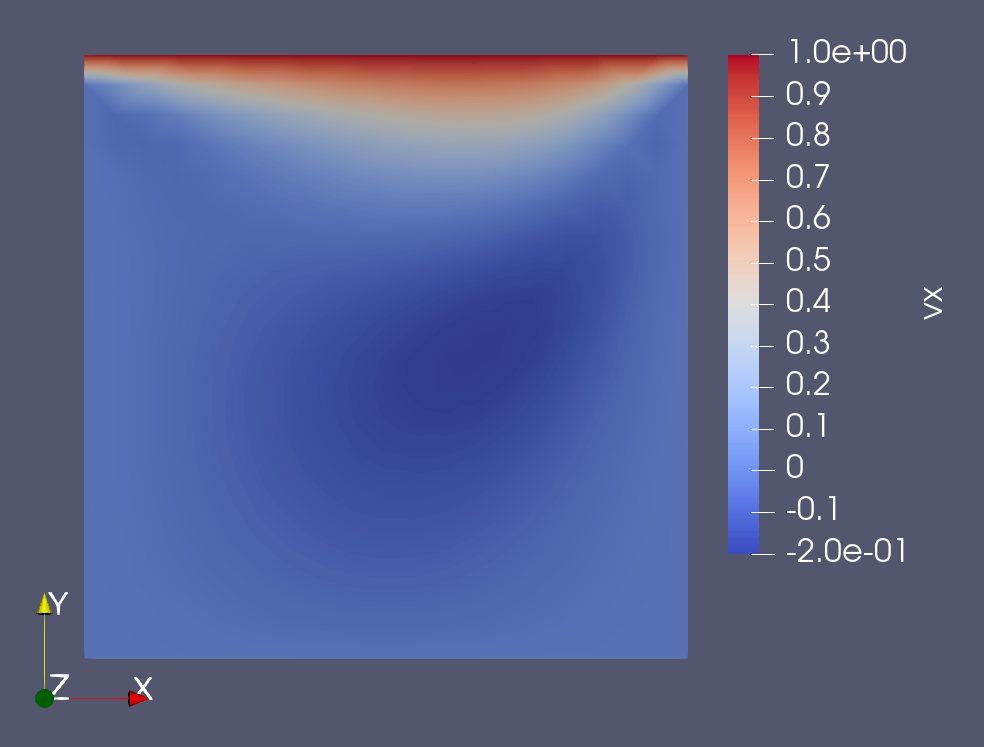
\includegraphics[width=200pt]{Figures/vx.png}}%
	\qquad
	\subfloat[\centering velocity in y-direction]{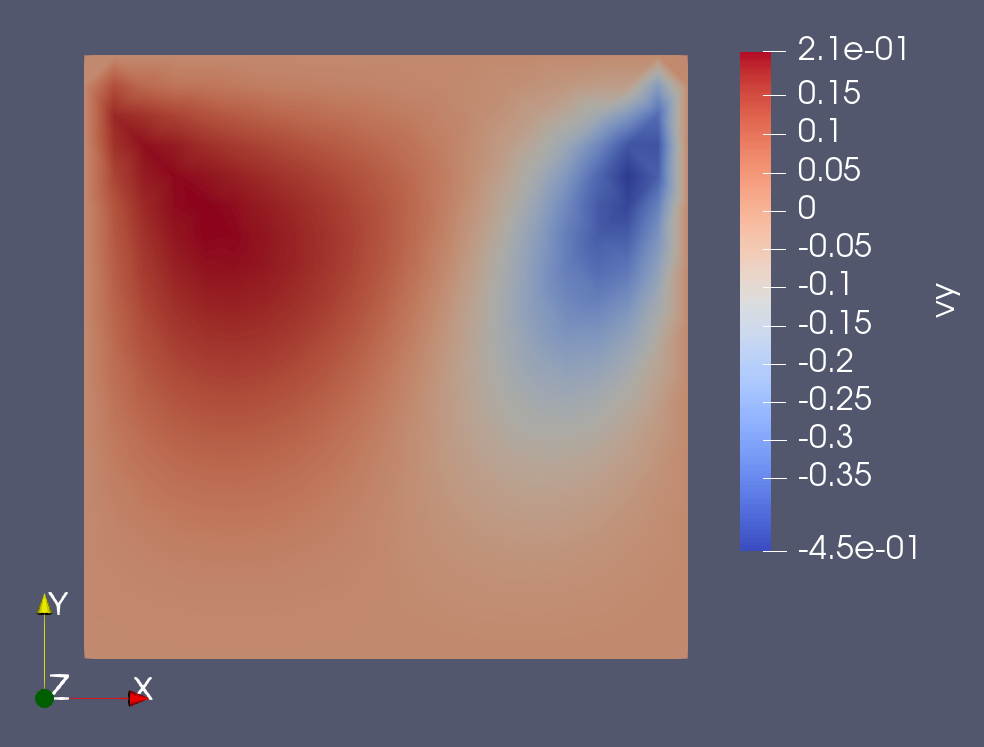
\includegraphics[width=200pt]{Figures/vy.png} }%
	\caption{velocity of flow in cavity for $Re=100$}%
	\label{fig_Rs1}%
\end{figure}
Pressure contour is presented in Figure \ref{fig_Rs2}.
\begin{figure}[htbp]
	\centering
	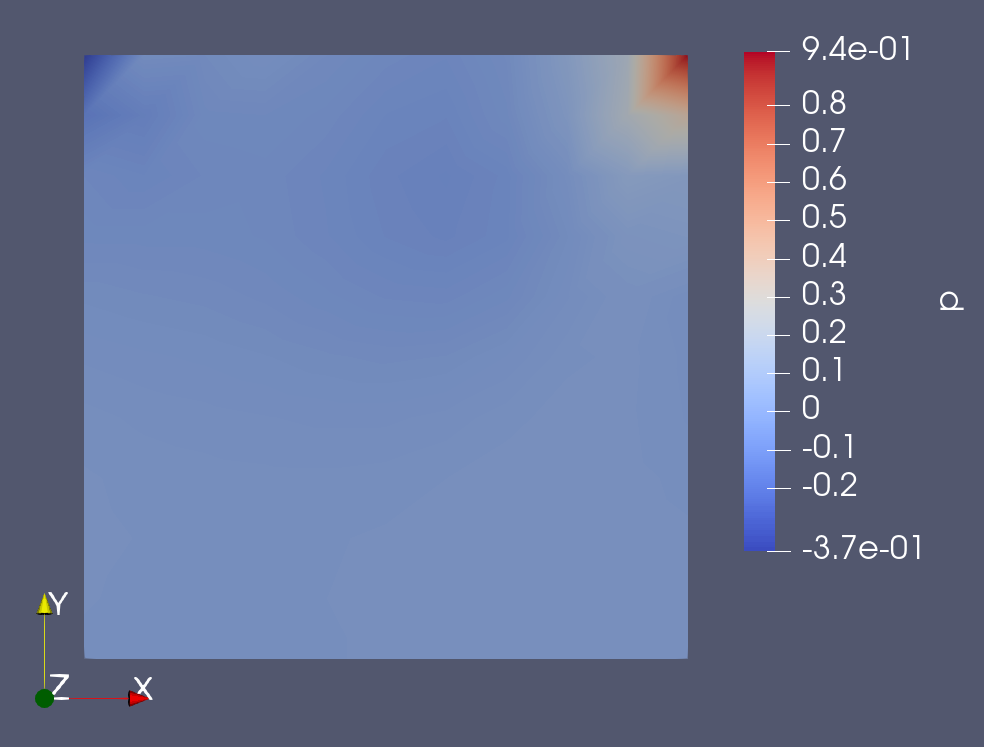
\includegraphics[width=250pt]{Figures/p.png}
	\caption{Pressure distribution in the domain for $Re=100$.}
	\label{fig_Rs2}
\end{figure}
\bibliographystyle{unsrt}
\bibliography{ref}
\end{document}
